\section{Past Experiments}
\paragraph{}
During the development of the Framework, many small tests have been developed, to both test the capabilities of the framework, and to be used in real studies.
Following some of those scenes are described.

\subsection[Influence of continuous depth]{Pilot Study: Influence of continuous depth on fatigue\label{FatiguePilot}}
\paragraph{}
Objective of the study is to quantify the effect of a continuous depth element on the time it takes participants to focus objects at various depths, and the change in refocus time with the progression of the experiment.

\begin{center}
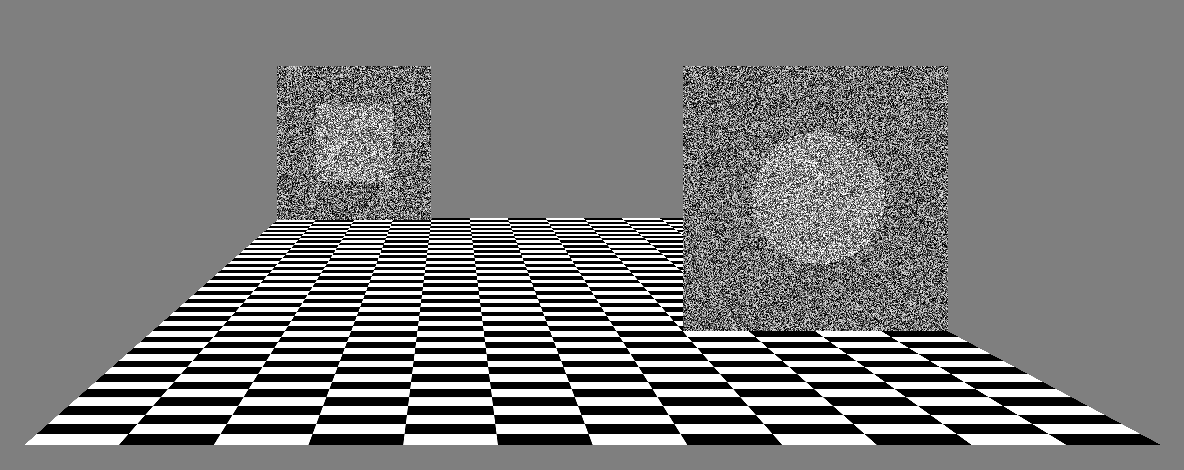
\includegraphics[width=7.5cm]{media/pilotFatigue.png}
\end{center}

\paragraph{Visual}
The test stimulus consists of a grey background (50\% grey), a continuous depth element (plane, checkerboard pattern, averaging in 50\% grey) and two random dot targets (approximately 50\% grey).
The targets show a shape which is either convex (coming out of the screen), or concave (going into the screen).
For the encoding details see section \ref{RDS}. The random pattern consists of eight shades of grey, of which the dark seven are used for the background, and the light seven for the foreground.

The random dot targets are resting on the plane, and border to either the left or the right border.
Each target can be at  one of three depth locations, at a separation of \unit[6]{cm}, \unit[0]{cm} and \unit[-6]{cm} (\unit[-3.1]{°}, \unit[0]{°}, \unit[3.1]{°}).
The targets itself are scaled up in the far position, and scaled down in the near position, to make their apparent size constant.

The image is back-projected on a screen by two projectors through circular polarisation filters.
The image height is \unit[0.79]{m}, it's width is \unit[1.3]{m} (\unit[36]{°} by \unit[22]{°} field of View).
The participant's head is at \unit[2]{m} distance of the screen, and observes the screen with polarised filter goggles. The room is dark.

\paragraph{Mechanics}
To asses the the effect of the continuous depth element, response time is logged.
The other variables are the depth location of the object, the change in depth measured in angular separation, the block number and the presence of the continuous depth element.

The expected input is randomized, so concave and convex targets should be similarly common.
The three depths and the two sides lead to 18 depth changes.

A cycle is built so that every depth change appears exactly once.
This is achieved by pre-computing three cycles and their inverses that visit each of the six positions three times, once from each of the three nodes on the other side.
Such a cycle has 18 steps, and 19 targets.
Cycles are picked at random out of the pre-computed cycles, randomly permuting the depth positions of right and left.
This gives 36 different permutations per cycle, and 216 different permutations overall.

Ten cycles form a block, either with or without continuous depth plane.
The start state is chosen by the tester to counterbalance it, the presence of the depth element in later blocks is alternated.
The whole test contains 12 blocks, 2280 targets.

Before the start, after the end, and after the first six blocks, a questionnaire is presented.
It starts with seven questions, with replies on a scale with six steps.
An other 16 questions require answers on a four step scale.


\subsection{Bisect test}
\paragraph{}
This is a helper test for the study on the influence of continuous depth on fatigue.
It's purpose is to find out the limits for stereo vision a person can reach.
During the first pilot study it became obvious that this depends heavily on the individual and it's experience in stereo viewing.

The test is visually very simple, it only shows one pixel plane with a stereogram.
The complexity is in the code.
(The name comes from the originally proposed algorithm.)

\paragraph{Mechanics}
Unlike usual tests it is not divided in blocks, and it is not limited by number of trials.
The tests are not balanced and pre-randomized either.

Instead the target moves it's position on screen and in depth dependent on the previous answers and the current position.
The target is moved to a near and far point in alternating order.
Five correct replies in a row allow the target point to move further away from the zero parallax plane,
a wrong answer makes it move closer.

The test is stopped when a predetermined maximal limit is reached or a limit is repeatedly failed to be reached.
During the test, voice output announces the current limit.


\section{Future Experiments}
\paragraph{}
\todo{content}

\section{Conclusions}
\paragraph{}
\todo{write}

\subsection{Thanks}
\paragraph{}
\todo{Add people who to thank}
\begin{itemize}
\item Steven Poulakos
\item Cary Kornfeld
\item Thomas Gross
\end{itemize}

